% % % % % % % % % % % % % % % % % % % % % % % % % % % % % % % % % % % % % % % %
% LaTeX4EI Template for Cheat Sheets                                Version 1.1
%
% Authors: Markus Hofbauer
% Contact: info@latex4ei.de
% Encode: UTF-8
% % % % % % % % % % % % % % % % % % % % % % % % % % % % % % % % % % % % % % % %


% ======================================================================
% Document Settings
% ======================================================================

% possible options: color/nocolor, english/german, threecolumn
% defaults: color, english
\documentclass[german]{latex4ei/latex4ei_sheet}

% set document information
\title{Physik}
\author{Darius Peters}                    % optional, delete if unchanged
\myemail{darius.peters@tum.de}           % optional, delete if unchanged
\mywebsite{www.latex4ei.de}          % optional, delete if unchanged

%custom packages
\usepackage{xcolor}

%custom settings
\titlespacing*{\subsection}{.5pt}{.5pt}{2pt}
\titlespacing*{\subsubsection}{0pt}{.5pt}{2pt}

%custom font
\renewcommand{\ttdefault}{cmtt}

% ======================================================================
% Begin
% ======================================================================
\begin{document}

% Title
% ----------------------------------------------------------------------
\maketitle   % requires ./img/Logo.pdf


% Allgemein
% ----------------------------------------------------------------------
\section{Allgemeines}

% Klassische Mechanik
% ----------------------------------------------------------------------
\section{Klassische Mechanik}
\begin{sectionbox}

\subsection{Bewegungen}
$x={\ir const.} \rightarrow v=0 \qquad v={\ir const.} \rightarrow a=0$ \\
$v=\dot{x} \qquad a=\ddot{x}$ \\
$x=\frac{1}{2}at^2+v_0t+x_0$ \\
$v=a\cdot t + v_0$
\subsubsection{Freier Fall}
$h=\frac{1}{2}gt^2 \qquad v_E=\sqrt{2gh}$\\
$\Delta t = \sqrt{2h/g}$
\subsubsection{Ebene}
$a=g\sin \alpha \qquad \Delta s = \frac{1}{2}g\sin \alpha$\\
$v_E=\sqrt{2gh}$
\subsubsection{Senkrechter Wurf}
$h=v_0t-\frac{1}{2}gt^2+h_0$\\
$v_M=\sqrt{0,5v_0} \qquad v^2 = v_0^2-2g(h_0-h)$\\
$v=v_0-g\cdot t$\\
$t_h=\frac{v_0}{g} \qquad x_h=\frac{v_0^2}{2g}$
\subsubsection{Waagrechter Wurf}
$v_y=gt \qquad v_x = v_0$\\
$s_y=h_0-\frac{1}{2}gt^2 \qquad s_x=v_0\cdot t_F$\\
$v=\sqrt{v_0^2+v_y^2}$\\
$s_y=h_0-\frac{g\cdot s_x^2}{2v_0^2}$
\subsubsection{Schräger Wurf}
$v_x=v_0\cos \alpha \qquad v_y=v_0\sin \alpha -gt$\\
$v_h=\sqrt{v_0^2-2gh}$\\
$s_x=v_0\cos \alpha t \qquad s_y=v_0 \sin \alpha t - \frac{1}{2} gt^2 +h_0$\\
$s_{x,\ir max}=\frac{v_0^2 \sin{2\alpha}}{g}$\\
$t_w=\frac{2v_0\sin \alpha}{g}$ \qquad
$h_{\ir max}=\frac{v_0^2 \sin^2 \alpha}{2g}+h_0$
\end{sectionbox}

\begin{sectionbox}
\subsection{Newton'sche Axiome}
\begin{enumerate}
	\item Masse ist träge. Jeder Körper behält seinen Bewegungszustand bei.
	\item $F=m\cdot a=\frac{\diff p}{\diff t}=\dot{p}$
	\item $F_{12}=-F_{21}$
\end{enumerate}
\textbf{Intertialsystem:} Koordinatensysteme die sich mit $v=\it const.$ zueinander bewegen.
\end{sectionbox}
\subsection{Kraft, Energie, Impuls}
\subsubsection{Kraft}
Federkraft: $F_F=-k(x-x_0)$ \\
Gewichtskraft: $F_G=mg$ \\
$F_N=mg\cos \alpha$ \\
$F_H=mg\sin \alpha$ \\
Zentripetalkraft: $F_Z=m\cdot \frac{v^2}{r}=m\omega^2r=p\omega$ \\
Reibungskraft: $F_R=\mu F_{(N)}=\mu m g \cos \alpha$
\subsubsection{Energie}
$E_{\ir kin}=\frac{1}{2}mv^2=\frac{p^2}{2m}$\\
$E_{\ir pot}=mgh$\\
$E_{F}=\frac{1}{2}k(x-x_0)^2$\\
$E_{\ir rot}=\frac{1}{2}I\omega^2$
\subsubsection{Arbeit}
$W=\Delta E=F\cdot s \cdot \cos \alpha$
\subsubsection{Leistung}
$P=
\underbrace{\frac{\Delta W}{\Delta t}}_{\text{mittlere Leistung}} 
= \, \underbrace{\frac{F\cdot \Delta s}{\Delta t}=F\cdot r}_{\text{momentane Leistung}}$\\
$\eta=\frac{E_{\it nutz}}{E_{\ir zu}}=\frac{P}{P}$
\subsubsection{Impuls}
$p_{\ir vorher}=p_{\ir nachher}$\\
$P=mv$\\
Mittlere Kraft: $\overline{F}=\frac{\Delta p}{\Delta t}$\\
Elastischer Stoß: $m_1v_1+m_2v_2=m_1u_1+m_2u_2$\\
Unelastischer Stoß: $m_1v_1+m_2v_2=(m_1+m_2)u$
\subsubsection{Raketengleichung}
$F=ma=\frac{\diff m}{\diff t}v_a+F_{\ir ext}$\\
$\vec{v}=\vec{v_0}+\vec{v_a}\ln | \frac{M_G}{m} | $\\
$m_0=M+m_a$
\subsection{Planetenbewegungen}
\subsubsection{Gravitation}
$U_{\ir pot}=-G\frac{m_E\cdot m}{r} \qquad r>r_E$\\
$\vec{F_G}=G\frac{m_1m_2}{r^2}\vec{e_r}$\\
$g=G\cdot \frac{m}{r^2}$\\
$W_G=Gm_1m_2(\frac{1}{r_1}-\frac{1}{r_2}$\\
$F_G \, || \, r \rightarrow M=r\times F=0$\\
\begin{sectionbox}
Satellit-Erde: $\frac{1}{2}m_Sv^2=G\frac{m_Sm_E}{R_E}$ \\
Stabile Umlaufbahn: $\omega_S=\sqrt{\frac{G\cdot m_E}{R_E^3}}\qquad v=\omega R_E$\\
Geostat. Umlaufbahn: $r_g=(G\cdot m_E \cdot \frac{T_g^2}{4\pi^2})^{\frac{1}{3}} \qquad h_g=r_g-R_E$
\end{sectionbox}
\subsubsection{Keplersche Gesetze}
\begin{itemize}
\item[1.] Keplersches Gesetz: Planetenbahnen sind Ellipsen um Stern in einem der beiden Brennpunkte\\
\item[2.] Keplersches Gesetz: In gleicher Zeit wird die gleiche Fläche an einer Bahn aufgespannt\\$\frac{dA}{dt} = \frac{1}{2} \v r \v v sin \alpha = \frac{1}{2}\v r \times \v v = \frac{1}{2}m|\v L| \Rightarrow$ Der Drehimpuls ist zeitlich konstant\\
\item[3.] Keplersches Gesetz: $\frac{T_1^2}{T_2^2} = \frac{a_1^3}{a_2^3}$ mit T: Umlaufzeit, a: Große Halbachse\\
\end{itemize}
\subsection{Drehungen}
\subsubsection{Drehmoment}
$M=F\times r=F\cdot r\cdot \sin \alpha$\\
$M=I\cdot \dot{\omega}=\frac{\diff L}{\diff t}$
\subsubsection{Trägheitsmoment}
Zylindermantel: $J = mr^2$ (Drehachse ist Körperachse)\\
Hohlzylinder: $J = \frac{1}{2}m(r_a^2+r_i^2)$ (Drehachse ist Körperachse)\\
Massive Kugel: $J = \frac{2}{5}mr^2$ (Drehachse durch Mittelpunkt)\\
\subsubsection{Drehimpuls}
$L=r\times p=I\cdot \omega = mrv$
\begin{sectionbox}
\subsection{Corioliskraft}
\begin{emphbox}
$\vec{F_c}=2m(v\times \omega)= 2m \cdot v \cdot w	\cdot \sin{(v\angle \omega)}$
\end{emphbox}
Rechte-Hand-Regel: Daumen: $\vec{v}$, Zeigefinger: $\vec{\omega}$ (von Süden nach Norden)\\
$a_c=-2(\omega \times v)=2v\omega$\\
$\Delta x= \frac{2}{3}\cos \beta \omega h \sqrt{\frac{2h}{g}}$\\
$\Delta y = -\omega^2R\cos \beta \sin \beta \frac{h}{g}$\\
%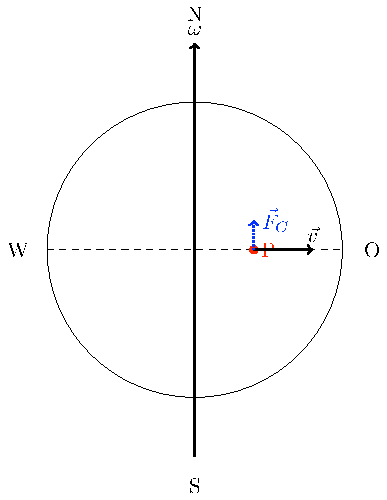
\includegraphics[width=0.25\columnwidth]{coriolis.pdf}
$R_E=\SI{6370}{\kilo \meter} \qquad r=R_E \cos \varphi \qquad \omega_E=\frac{2\pi}{86400\si{\second}}$\\
$F_C$: Auf der Nordhalbkugel nach rechts. Auf der Südhalbkugel nach links.
\end{sectionbox}

% Harmonische Schwingungen
% ----------------------------------------------------------------------
\section{Harmonische Schwingungen}
$x(t)=A_0\cos(\omega t + \varphi)$ \\
$\dot{x}(t)=-A_0\omega\sin(\omega t + \varphi)$\\
$\ddot{x}(t)=-A_0\omega^2\sin(\omega t + \varphi)$
\subsection{Frei ungedämpft}
Bewegungsgleichung: $\ddot{x}+\omega_0^2x=0$\\
$f_0=\frac{\omega_0}{2\pi} \qquad y_0=\frac{mg}{k} \qquad v_0 = \hat{x}\sqrt{\frac{k}{m}}$
\subsubsection{Federpendel}
$\omega_0^2=\frac{\text{Rücktreibende Kraft}}{\text{Einheitsmasse} \times \text{Einheitsauslenkung}}=\frac{k}{m} \rightarrow \omega = \sqrt{\frac{k}{m}}$\\
$A_0=v_0\sqrt{\frac{m}{k}}=\frac{v_0}{\omega_0}$\\
Bewegungsgleichung: $\ddot{x}+\frac{k}{m}x=0$
\subsubsection{Fadenpendel}
Kleinwinkelnäherung: $\alpha << 1$\\
$\omega_0=\sqrt{g}{l}$\\
$l=\frac{T_0^2g}{4\pi^2} \qquad h=l-l\cos \alpha$\\
$A_0 = v_0 \sqrt{\frac{l}{g}} \qquad E_{\ir ges} = mgl(\frac{3}{2}-\cos \alpha)$\\
Bewegungsgleichung: $\ddot{x}+\frac{g}{l}x=0$
\subsubsection{Torisionsschwingungen}
$\omega_0 = \sqrt{\frac{k_t}{I}}=\sqrt{\frac{k_t}{mr^2}}$\\
$I=\frac{T_0^2}{4\pi^2}k_t \qquad T_0=2\pi \sqrt{\frac{I}{k_t}}$\\
Bewegungsgleichung: $\ddot{x}+\frac{k_t}{I}x=0$
\subsection{Frei gedämpft}
Stokesche Reibungskraft: $F_R=-6 \pi \eta R \vec{v}=-2m\delta\vec{v}$\\
Bewegungsgleichung: $\ddot{x}+2\delta \dot{x}+\omega_0^2x=0$\\
 Resonanzfrequenz $\omega'=\sqrt{\omega_0^2-\delta^2}$ \\
 $\delta = \frac{b}{2m}=\frac{3\pi \eta R}{m}$\\
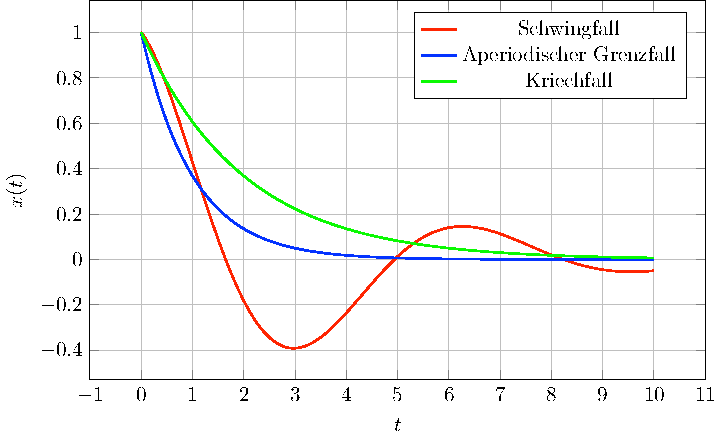
\includegraphics[width=.9\columnwidth]{img/Schwingungen.pdf}
\subsubsection{Schwingfall}
$\omega_0^2>\delta^2$\\
$\omega'=\sqrt{\omega_0^2-\delta^2}<\omega_0$\\
$x(t)=Ae^{-\delta t}\cos(\omega't)$
\subsubsection{Aperiodischer Grenzfall}
$\omega_0^2=\delta^2$\\
$\omega'=0$\\
$x(t)=Ae^{-\delta t}\cdot (1+\delta t)$
\subsubsection{Kriechfall}
$\omega_0^2<\delta^2$\\
$\omega'=i\delta \pm i\sqrt{\delta^2-\omega_0^2}$
$x(t)=A_1e^{-(\delta+\sqrt{\delta^2-\omega_0^2})t}+A_2e^{-(\delta - \sqrt{\delta^2-\omega_0^2})t}$
\subsection{Erzwungen gedämpft}
Bewegungsgleichung: $\ddot{x}+2\delta \dot{x}+\omega_0^2x=F_0e^{-i\Omega t}$\\
%Resonanzfrequenz $\Omega_{\ir res}=\sqrt{\omega_0^2-2\gamma^2}$\\%
$\hat{x}(t)=Ae^{i(\Omega t + \varphi}$\\
$A(\Omega)=\frac{F_0/m}{\sqrt{(\omega_0^2-\Omega^2)^2+(\frac{b\Omega}{m})^2}}$\\
\textbf{Resonanzfälle:}
\begin{enumerate}
	\item $\Omega < \omega_0$\\
		$A\rightarrow \frac{F_0m^{-1}}{\omega_0^2}=\frac{F_0}{k}$\\
		$\Delta \varphi = 0 \qquad \Omega \rightarrow 0$
	\item $\Omega \approx \omega_0$ (Katastrophe)\\
		$A_{\ir max}=frac{F_0}{b\omega_0}=\frac{F_0/m}{2\delta \sqrt{\omega_0^2-\delta^2}} \rightarrow \infty$\\
		$\Omega_{\ir max}=\sqrt{\omega_0^2-\frac{1}{2}(\frac{b}{m})^2}=\sqrt{\omega_0^2-2(\frac{3\pi \eta R}{m})^2}\rightarrow \omega_0$
		$\Delta \varphi = \frac{\pi}{2} \qquad \delta \rightarrow 0$
		\item $\Omega > \omega_0$\\
		$A\rightarrow 0$\\
		$\Delta \varphi = \pi \qquad \Omega \rightarrow \infty$
\end{enumerate}

% Wellen
% ----------------------------------------------------------------------
\section{Wellen}
\subsection{Allgemeines}
Allgemeine Wellengleichung: $\frac{1}{c^2}\frac{\delta^2u}{\delta t^2}=\Delta u$\\
$\frac{c}=\lambda \cdot f=\frac{\omega}{k}=\frac{x}{\Delta t}$\\
$\omega = 2\pi f=\frac{2\pi}{T} \qquad k=\frac{2\pi}{\lambda}=\frac{\omega}{c}$
Funktion: $y(x,t)=\hat{y}\sin(kx - \omega t + \phi)$
\subsection{Doppler-Effekt}
\begin{enumerate}
	\item Beobachter \textbf{bewegt}, Quelle \textbf{ruht}\\
		Annäherung: $f_B=f_Q(1+\frac{v_B}{c}$\\
		Entfernung: $f_B=f_Q(1-\frac{v_B}{c}$
	\item Beobachter \textbf{ruht}, Quelle \textbf{bewegt}\\
		Annäherung: $f_B=\frac{f_Q}{1-v_Q/c}$\\
		Entfernung: $f_B=\frac{f_Q}{1+v_Q/c}$
	\item Beobachter \textbf{bewegt}, Quelle \textbf{bewegt}\\
		$f_B = f_Q \frac{c \, \underset{\textcolor{green}{-}}{\textcolor{red}{+}} \, V_B}{c \, \underset{\textcolor{green}{+}}{\textcolor{red}{-}} \, V_Q} \qquad \text{Q} \, \underset{\textcolor{green}{\leftarrow} \textcolor{green}{\rightarrow}}{\textcolor{red}{\rightarrow} \textcolor{red}{\leftarrow}} \, \text{B}$\\
		$f_B = f_Q \frac{c \, \underset{\textcolor{cyan}{-}}{\textcolor{purple}{+}} \, V_B}{c \, \underset{\textcolor{cyan}{-}}{\textcolor{purple}{+}} \, V_Q} \qquad \text{Q} \, \underset{\textcolor{cyan}{\rightarrow} \textcolor{cyan}{\rightarrow}}{\textcolor{purple}{\leftarrow} \textcolor{purple}{\leftarrow}} \, \text{B}$
	\item Quelle \textbf{bewegt} ($v>1 \ir Ma$)\\
		$\sin \alpha=\frac{\diff w}{\diff s}=\frac{c_s t}{v_Qt}=\frac{1}{\ir Ma}$
\end{enumerate}
\subsection{Schwebung}
Tritt auf bei $f_1\approx f_2$ ($f_1 \neq f_2$)\\
$f_S=|f_1-f_2| \qquad f_R= \frac{f_1+f_2}{2}$\\
$y(t)=\underbrace{2\hat{y}\cos(2\pi\frac{f_1-f_2}{2}\cdot t)}_{\text{Amplitudenfaktor}} \cdot \underbrace{\sin(2\pi \frac{f_1+f_2}{2}\cdot t)}_{f_R} $\\ 
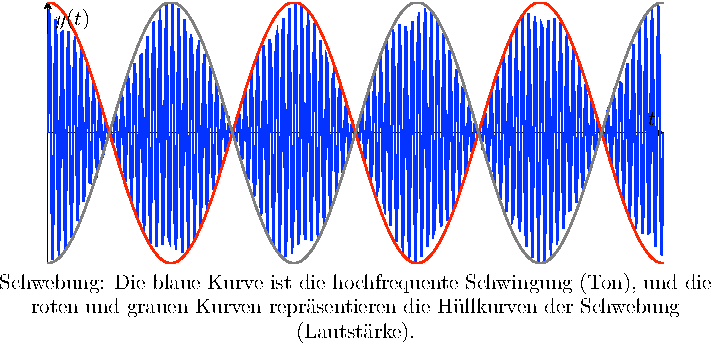
\includegraphics[width=.9\columnwidth]{Schwebung_crop.pdf}
\subsection{Gekoppelte Wellen}
\begin{enumerate}
    \item \textbf{Gleichphasig} $(x_1 = x_2)$ : $\omega_1 = \omega_0 = \sqrt{\frac{K}{m}}$
    
    \item \textbf{Gegenphasig} $(x_1 \neq x_2)$ : $\omega_2 = \sqrt{\omega_0 + \frac{2K_{12}}{m}}$
    
    \item \textbf{Allgemein}\\
    $x_1(t) = x_0 \cos\left( \frac{\omega_0 + \omega_2}{2} t \right) \cos\left( \frac{\omega_0 - \omega_2}{2} t \right)$\\
	$x_2(t) = x_0 \sin\left( \frac{\omega_0 + \omega_2}{2} t \right) \sin\left( \frac{\omega_0 - \omega_2}{2} t \right)$
\end{enumerate}
\subsection{Interferenz}
$f_1=f_2 \qquad A_1 = A_2 \qquad \varphi_1 \neq \varphi_2$\\
Konstruktiv: $\Delta \varphi = 2\pi \cdot n$\\
Destruktiv: $\Delta \varphi = (2n+1)\pi$\\
\textbf{Allgemein:}
\begin{itemize}
	\item Gangunterschied $\Delta s = a\sin \alpha = \frac{x}{n}\sin \alpha$
	\item Phasendifferenz $\varphi = 2\pi \frac{\Delta}{\lambda}=2\pi a \frac{\sin \alpha}{n\lambda}$
	\item Winkel Max: $\sin \alpha_n = \pm n \lambda/a$
	\item Winkel Min: $\sin \alpha_n = \pm (n+\frac{1}{2})\lambda / a$
\end{itemize}
\subsubsection{Doppelspalt}
Int max: $\Delta s = \lambda n$ (Konstruktiv)\\
Int min: $\Delta s = (2n+1)\frac{\lambda}{2}$ (Destruktiv)\\
$\Delta s = a \sin \alpha' \approx a \frac{x}{d}$\\
Kleinwinkelnäherung: $frac{x}{d}\approx \tan \alpha \approx \sin \alpha \approx \alpha \approx \alpha'$\\
$\Rightarrow \frac{\Delta s}{a} = \frac{x}{d}$
\subsubsection{Gitter}
Hauptmaximum: $\sin \alpha_{\ir max} = m\frac{\lambda}{d}$\\
Einfachspalt: $\sin \alpha_{\ir min} = \pm m \frac{\lambda}{a}$
\subsection{Reflexion und Wellen in einem Medium}
Festes Ende: $\varphi = \pi$ (Knoten am Ende)\\
Loses Ende: $\varphi = 0$ (Bauch am Ende)\\
Bei jeder zusätzlichen Oberschwingung wird die Welle gestaucht, sodass die obigen Bedingungen weiterhin gelten (Tipp: Skizze der Welle im Medium zeichnen)


% Optik
% ----------------------------------------------------------------------
\section{Optik}
\begin{sectionbox}
\subsection{Rexlexion und Brechnung}
$f_m \cdot \lambda_m = c_m$ \qquad
$\lambda_m = \frac{\lambda_0}{m}$\\
Berchnungsindex $n=\frac{c_0}{c_m}$
\subsubsection{Brechungsmöglichkeiten}
\begin{enumerate}
\item[A)] \textbf{zum Lot} (dünn nach dicht)\\
$\sin \alpha > \sin \beta$ \qquad $c_1 > c_2$
\item[B)] \textbf{vom Lot} (dicht nach dünn)\\
$\sin \alpha < \sin \beta$ \qquad $c_1 < c_2$
\end{enumerate}
\subsubsection{Gesetz von Snellius}
$\frac{\sin \alpha}{\sin \beta} = \frac{n_2}{n_1} = \frac {c_1}{c_2}$
\subsubsection{Totalreflexion}
Nur möglich wenn $n_1 > n_2$ und $\theta > \theta_{\ir krit}$ \\
$\theta_{\ir krit} = \arcsin \frac{n_2}{n_1}$\\
Einfallswinkel = Ausfallswinkel
\end{sectionbox}

\begin{sectionbox}
\subsection{Linsen}
Linsengleichung
\begin{emphbox}
$D=\frac{1}{f}=\frac{1}{g}+\frac{1}{b}$	
\end{emphbox}
Vergößerung: $V=\frac{B}{G}= - \frac{b}{g}=\frac{\tan \alpha}{\tan \alpha_0}$\\
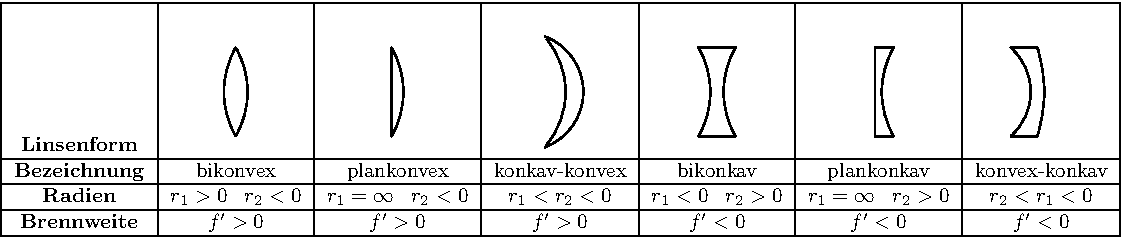
\includegraphics[width=\columnwidth]{img/Linsen_crop.pdf}
\subsubsection{Hohlspiegel}
$f=\frac{r}{2}$ \qquad $V=\frac{B}{G}= - \frac{n_1b}{n_2g}$ \\
$D=\frac{n_1}{g}+\frac{n_2b}=\frac{n_2-n_1}{r}$\\
$g\rightarrow \infty: b=f_B=\frac{n_2r}{n_2-n_1}$\\
$b\rightarrow \infty: g=f_G=\frac{n_1r}{n_2-n_1}$\\
%Bild
\subsubsection{Dünne Linsen}
$\frac{1}{f}=\frac{1}{g}+\frac{1}{b}=(\frac{n_2}{n_1}-1)(\frac{1}{r_1}-\frac{1}{r_2})$\\
\textbf{Konvexe Linse (Sammellinse)} \\
$V_{\ir sammel}= \frac{b}{g}=\frac{b-f}{f}$\\
Korrektur von Weitsichtigkeit \\
%Bild
\textbf{Abbildung}
\begin{itemize}
	\item $\infty > g > 2f \Rightarrow 2f>b>f \quad G>B$ (real und invertiert)
	\item $g=2f \Rightarrow 2f=b \quad G=B$ (real und invertiert)
	\item $2f>g>f \Rightarrow \infty >b>2f \quad G<B$ (real und invertiert)
	\item $0<g<f \Rightarrow -b>g \quad G<B$ (virtuell und aufrecht)
\end{itemize}
\textbf{Konkave Linse (Zerstreuungslinse)}\\
Korrektur von Kurzsichtigkeit\\
\textbf{Abbildung}
\begin{itemize}
\item[$\rightarrow$] Bild immer zwischen Brennpunkt und Linse
\item[$\rightarrow$] Bild immer verkleinert ($G>B$)
\item[$\rightarrow$] Bild immer virtuell und aufrecht
\end{itemize}
\subsubsection{Dicke Linsen}
$\frac{1}{f}=(\frac{n}{n_0}-1)(\frac{1}{r_1}-\frac{1}{r_2}+\frac{(n-n_0)d}{n\cdot r_1 \cdot r_2})$\\
$h_1=-\frac{f(n-1)d}{n\cdot r_2}$ \qquad $h_2=-\frac{f(n-1)d}{n\cdot r_1}$
\subsubsection{Linsensysteme}
\begin{itemize}
	\item \textbf{Lochkamera} \\
		$S=\frac{D(b+g)}{g}$
	\item \textbf{Lupe} \\
		$V=\frac{\tan \alpha_L}{\alpha_0}=\frac{G/f}{G/s_0}=\frac{s_0}{f}$ mit $s_0=\SI{25}{\centi \meter}$
	\item \textbf{Fernrohr} \\
		$V=\frac{f_{ob}}{f_{ok}}$, $g\approx \infty$, $b\approx f$ \\
		$V_T=\frac{f}{g-f}=\frac{b-f}{f}\approx 0$
	\item \textbf{Mikroskop} \\
		$V=V_{ok}\cdot V_{ob}=\frac{(d-f_{ob})s_0}{f_ob \cdot f_ok}=-\frac{l}{f_{ob}}\cdot \frac{s_0}{f_{ok}}$
	\item \textbf{Auflösung Mikroskop} \\
	mit Spalt b: $\delta_{\ir{min}} = \alpha = \arcsin\frac{\lambda}{b} \approx \frac{\lambda}{b}$ (Abbé Limit)\\
	für runde Linse mit Durchmesser D: $\delta_{\ir{min}} = D\cdot\sin\alpha = 1,22\frac{\lambda}{D}$ (Rayleigh-Kriterium)\\
\end{itemize}
\end{sectionbox}
\subsection{Absorption und Polarisation}
\begin{sectionbox}


\subsubsection{Absorption}
Berchungsindex mit Absorption: $n\rightarrow \tilde{n}=n-i\kappa$\\ 
Re($\tilde{n}$)$=n$: Brechung \\
Im($\tilde{n}$)$=\kappa$: Absorption \\
Absorptionsgesetz von Lambert-Beer: $I=I_0e^{-\alpha \cdot d}=I_0e^{-\frac{2\omega}{c}\kappa d}$

\subsubsection{Polarisation}

Gesetz von Malus (für polarisiertes Licht): $I = I_0 \cos^2 \alpha$

Für unpolarisiertes Licht gilt nach einem Polarisationsfilter: $I = \frac{I_0}{2}$

\end{sectionbox}

%Malus, Lambert-Beer, etc.

% Hydromechanik
% ----------------------------------------------------------------------
\section{Hydromechanik}
\begin{sectionbox}
Dichte: $\rho=\frac{m}{V}$\\
Homogener Druck: $P=\frac{F_N}{A}$\\
Kompressibilität: $\kappa = -\frac{1}{\Delta P}\cdot \frac{\Delta V}{V}$\\
Kompressionsmodul: $K=\frac{1}{\kappa}$\\
$R_E= \frac{V\cdot \rho \cdot L}{\eta}$

\subsection{Hydraulische Presse}
$\frac{F_1}{A_1}=\frac{F_2}{A_2}$ \\
$\frac{\Delta x_1}{\Delta x_2}=\frac{F_2}{F_1}?\frac{A_2}{A_1}$
\subsection{Kontinuitätsgleichung}
$\dot{m}=\rho_1 A_1 \vec{v_1}=\rho_2 A_2 \vec{v_2}$\\
$\dot{V}=\frac{\dot{m}}{\rho}=A\vec{v}$

\subsection{Bernoulli Gleichung}
$\underbrace{p}_{\text{statischer Druck}} 
+ \underbrace{\frac{1}{2} \rho v^2}_{\text{dynamischer Druck}} 
+ \underbrace{\rho gh}_{\text{hydrostatischer Druck}} = \ir{const.}$\\
$p_{\ir B,1}\stackrel{!}{=}p_{\ir B,2}$
(Energieerhaltung der Hydromechanik)

\subsection{Torricelli}
$\vec{v_2}=\sqrt{2(gh+\frac{P_1-P_2}{\rho})}$\\
$P_1=P_2=P_\infty = \SI{10e5}{\pascal}$

\subsection{Gesetz von Hagen-Poiseulle}
Strömung durch ein Rohr\\
$\dot{V}=\frac{\diff V}{\diff t}=\frac{\pi (P_1-P_2)}{8\eta \cdot l}R^4$\\
$v(r)=\frac{P_1-P_2}{4\eta \cdot l}(R^2-r^2)$

\subsection{Strömungen}
\begin{enumerate}
	\item \textbf{Turbulente Strömung:} \\
		Größe Geschwindigkeiten, geringe innere Reibung, hohe Reibung an den Wänden.\\
			Newtonsches Reibungsgesetz:\\
			$F_R=\eta A \frac{\diff v}{\diff x}$\\
			$\eta=\eta_0e^{T/T_0}$ \\
			$R_e >> 1$: $F_w=F_R+F_D=c_w \cdot A \cdot \frac{\rho v^2}{2}$
	\item \textbf{Laminare Strömung:} \\
			$R_e<1$: Stokesche Reibung\\
			$F=b\cdot v = 6\pi \eta r v$
\end{enumerate}
\textbf{Hydrostatisches Paradoxon:} Druck am Boden hängt nur von Füllhöhe, nicht Form/Menge ab.\\
\textbf{Hydrodynamisches Paradoxon:} Gleichgewicht bei $mg=\frac{1}{2}\rho v^2 A$. Wenn $v$ steigt, dann fällt $P$.
\end{sectionbox}


% Thermodynamik
% ----------------------------------------------------------------------
\section{Thermodynamik}
%aus alter LaTeX FS + Entropie und ein paar kleine Änderungen
\begin{sectionbox}
\textbf{Ideale Gasgleichung:} 
\begin{emphbox}
$p \cdot V = \nu \cdot R \cdot T$ 
\end{emphbox}
Stoffmenge $\nu = \frac{m}{M}$ \qquad $M$: mol. Masse\\
\textbf{Wärmemenge Q} \\
$Q=C_p(T_2-T_1)=c \cdot m \cdot \Delta T$ \\ $c$: spez. Wärmekapazität \\

\textbf{Gesetz von Boyle + Mariotte} \\
für $N=\ir const$ und $T=\ir const.$ gilt: $p_1V_1=p_2V_2$ \\

\textbf{2. Gesetz von Gay Lussac} \\
feste Gasmenge; $V=\ir const.$\\
$\frac{p_1}{T_1}=\frac{p_2}{T_2}$ \\

\textbf{Thermodynamische Systeme:}
\begin{itemize}
	\item \textbf{Offen} (Verbrennungsmotor) \\
		Austausch von Materie, Arbeit, Wärme
	\item \textbf{Geschlossen} (Stirlingmotor) \\
		Austausch von Arbeit, Wärme
	\item \textbf{Abgeschlossen} (Thermoskanne) \\
		kein Austausch mit der Umgebung
		
\end{itemize}

\textbf{Mittlere kin. Energie eines Gases} \\
$\overline{E}_{\ir kin}=\frac{3}{2}k_B \cdot T$ \\

\textbf{Gesamte Translationsenergie} \\
$U=\frac{3RT}{2M}$ \, $U$: innere Energie

\textbf{Energien}
$\Delta U = \int_{T_1}^{T_2} c \, \diff T$\\
$W=-\int_{V_1}^{V_2} p \diff V$ \qquad $\partial W= -p \cdot \partial V$

\end{sectionbox}

\subsection{Hauptsätze der Thermodynamik}

\begin{itemize}
\item[0.] Zwei Körper im thermischen Gleichgewicht zu einem dritten\\ $\rightarrow$ Alle stehen untereinander im Gleichgewicht\\
\item[1.] $\Delta U = \Delta Q + \Delta W \rightarrow $ Es gibt kein Perpetuum mobile erster Art - Maschine mit $>$100\% Wirkungsgrad\\ \\
$\textbf{Verschiedene Möglichkeiten für Zustandsänderung:}$
%TODO BESSERE LISTE %TODO
\begin{sectionbox}
$\textbf{a)}$ Isobarer Prozess, $p =$ const.\\ $\rightarrow$ im idealen Gas ist $C_p$ konstant $\Rightarrow Q_{12} = C_p \Delta T$\\
$\textbf{b)}$ Isochorer Prozess: $V =$ const.\\ $\rightarrow$ im idealen Gas ist $C_v$ konstant $\Rightarrow Q_{12} = \Delta U$\\
$\textbf{c)}$ Isothermer Prozess: $T =$ const.\\ $\Rightarrow$ $W_{12} = -Q_{12}$ %Umsetzung der Wärmezufuhr in Arbeit $\Rightarrow W_{12} = \\$
$ =\nu RT \ln\frac{V_1}{V_2}$
\\Freiwerdende Wärme: $Q_{12} = -W_{12}$\\
$\textbf{d)}$ Adiabatischer Prozess: $\Delta Q = 0$\\
%TODO Isochorer Prozess, Isothermer Prozess, adiabatischer Prozess verbessern\\
In differentieller Schreibweise: $\partial U = \partial W + \partial Q $\\
$\frac{T_2}{T_1}=({\nu_1}{\nu_2})^{\gamma -1}$\\
$\Delta W = \Delta U = \eta \cdot C_u(T_2-T_1)$
\end{sectionbox}
\item[2.] Thermische Energie ist nicht in beliebigem Maße in andere Energiearten umwandelbar. $\eta < 1$
\item[3.] Nernst'sches Theorem: $\lim_{T \rightarrow 0} S(T) = 0$ (Entropie bei 0 K ist 0)\\
\end{itemize}

\subsection{Adiabatengleichung}
$p\cdot V^\kappa = \ir const.$ \qquad $T\cdot V^{\kappa -1} = \ir const.$ \\
Carnotscher Kreisprozess: Idee der Wärmekraftmaschine\\
Wirkungsgrad $\eta = \frac{\vert W\vert}{Q_{12}}$, $\eta_{\text{Carnot}} = \frac{T_2-T_1}{T_2} < 1$\\
Entropieänderung ist null

\subsection{Entropie}
Maß der Unordnung in einem System
\begin{itemize}
	\item Es ist wahrscheinlicher, dass die Unordnung zunimmt
	\item Kann spontan nur in eine Richtung ablaufen
\end{itemize}
$\Rightarrow$ Entropie kann nur steigen oder konstant bleiben\\ \\

$S=-k_B\sum p_i \ln p_i$ \\ 
$p_i$: Wahrscheinlichkeiten der Mikrozustände\\
$\partial S = \frac{\partial Q_{rev}}{T}$\\
Ideales Gas: $\Delta S= \int \partial S = n \cdot c_v \ln \frac{T_2}{T_1}+n\cdot R \ln \frac{V_2}{V_1}$



% Quantenmechanik
% ----------------------------------------------------------------------
\section{Quantenmechanik}
\subsection{Stefan Boltzmann}
\begin{emphbox}
$P=\epsilon \sigma A T^4 = 4 \pi r^2 E_0$
\end{emphbox}
Für schwarze Körper gilt: $\epsilon = 1$\\
Wienscher Verschiebungssatz: $\lambda_{\ir max}=\frac{\num{2,898e-3}}{T} \si{\kelvin \meter}$
\subsection{Weiteres zur Quantenmechanik}
Licht wird abhängig von der Frequenz in Quanten der Energie $h\cdot f$ emittiert und absorbiert.
% ======================================================================
% End
% ======================================================================
\end{document}
